\chapter{Choix techniques} \label{chap:choix_techniques}

Ce chapitre détaille les principaux choix techniques.
Après avoir présenté la vue d'ensemble de l'architecture, nous présentons les 3 difficultés majeures:
l'installation de \component{jbpmmicroscope}, la mise à disposition des banques et
l'installation des logiciels métier.

\section{Vue d'ensemble}

La vue d'ensemble de l'architecture est présentée dans la~\autoref{fig:architecture}.

\begin{figure}[htp]
    \centering
    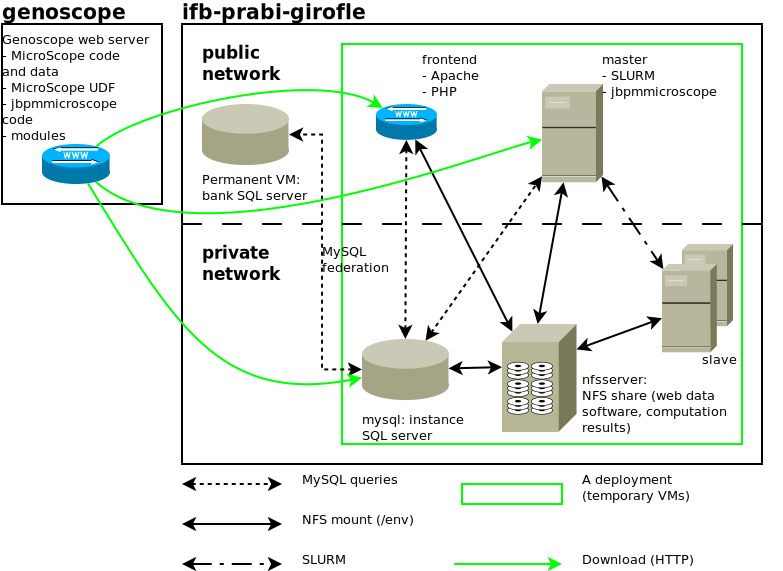
\includegraphics[width=\linewidth]{../Architecture}
    \caption{Schéma de l'architecture de MicroCloud.}
    \label{fig:architecture}
\end{figure}

Un des buts est de mimer ce qui est fait au Genoscope
c'est-à-dire que:
\begin{enumerate}
    \item Les différents composants (serveur web, serveur de BD, etc.) tournent sur des machines séparées.
    \item Les calculs tournent sur des machines séparées: l'architecture contient donc un cluster (basé sur SLURM).
    \item Les machines partagent un disque commun (qui est utilisé pour accéder aux données et aux logiciels).
          Le répertoire \path{/env} est similaire au répertoire de même nom sur le cluster \hostname{etna}
          afin de simplifier l'installation de MicroScope.
\end{enumerate}\vspace*{\baselineskip}

Une des différences est que le serveur \component{jbpmmicroscope} tourne
sur la machine frontale du cluster.
Ceci a été fait pour diminuer légèrement le nombre de composants
(car il faudrait faire un nouveau composant capable de soumettre des jobs sur \SScomponent{master}).
De plus, il n'est pas exclu que cela aurait pu nécessiter d'autres modifications dans \component{jbpmmicroscope}.

L'autre différence est l'utilisation d'une machine partagée pour fournir l'accès aux banques (voir~\autoref{sec:acces_banques}).
Il y a donc 2 serveurs de bases de données dans MicroCloud:
\begin{itemize}
    \item Un serveur MySQL propre à chaque instance.
    \item Un serveur MySQL partagé sur la VM permanente.
\end{itemize}\vspace*{\baselineskip}

Lors du déploiement, les VM téléchargent des fichiers (code et données) depuis le serveur web du Genoscope (voir~\autoref{chap:deploiement_VM}).
Ces fichiers sont crées par le module \micWEBdeployVer{} (voir~\autoref{chap:micwebdeploy}).
Le gros du travail est fait dans les scripts de la phase Deployment (script \script{04\_Deployment.sh} de chaque composant SlipStream).
Ceci a été fait pour simplifier les scripts d'installation (c'est-à-dire avant la phase de déploiement)
et ne pas fixer les versions de MicroScope à ces étapes.

\section{Installation de \component{jbpmmicroscope}} \label{sec:installation_jbpmmicroscope}

\subsection{Défis}

L'installation de \component{jbpmmicroscope} est très difficile pour plusieurs raisons:
\begin{enumerate}
    \item \emph{Manque de documentation.} Il n'a pas de documentation sur le projet donc tous les points suivants sont difficiles à modifier.
    \item \emph{La configuration est dans le code.} La configuration du serveur SQL à utiliser est codée dans les fichiers jar et war lors de la compilation.
           Ainsi, les différentes instances (\mageInstance{microscope}, \mageInstance{labscope}, \mageInstance{dietetic}, \mageInstance{coliscope}) sont compilées avec des profils maven spécifiques.
           En théorie, il est possible de ne pas faire cela dans \component{Tomcat}.
    \item \emph{Organisation du projet confuse.} Le projet est découpé en 3 sous-projets maven (\component{jbpmmicroscope-server}, \component{jbpmmicroscope-client} et \component{jbpmmicroscope-commons}\footnote{Nous laissons de côté \component{jbpmmicroscope-web-services} qui apparemment n'a jamais marché.}).
          Cependant, la distinction est assez floue et le fichier XML qui décrit les WF est à un autre endroit (\path{src}).
          De plus, il semble que les sources de \component{jBPM 3.2.3} lui-même soient incluses dans le projet.
    \item \emph{Utilisation de \component{jBPM 3.2.3}.} Cette version de \component{jBPM} est obsolète depuis longtemps.
    \item \emph{Utilisation de XSLT 2.0.} La transformation du fichier XML qui décrit tous les WF en langage JPDL se base sur XSLT 2.0.
          Or cette version de la norme est peu répandue.
          Par exemple, le plugin \component{Orange Volt} utilisé dans nos procédures est obsolète depuis longtemps.
\end{enumerate}

\subsection{Revue des solutions}

\subsubsection{Tentative d'installation de versions plus récentes de jBPM}

Nous avons testé l'installation de versions plus récentes de \component{jBPM} (sans la surcouche \component{jbpmmicrosope}).
Voir \href{https://intranet.genoscope.cns.fr/agc/redmine/documents/88}{les documents sur le projet Redmine}.
Globalement, nous avons réussi à installer \component{jBPM} séparément mais cela n'aidait pas
car la manière d'installer \component{jbpmmicroscope} par dessus n'est pas claire.

\subsubsection{Reprise des développements}

Nous avons envisagé la reprise des développements de \component{jbpmmicroscope}.
En particulier, nous nous sommes intéressés à:
\begin{itemize}
    \item Mieux séparer le client et le serveur par exemple en utilisant les API du serveur (bien que cela ne soit pas très clair).
    \item Ne pas inscrire la configuration dans le code (en utilisant des mécanismes de configuration des serveurs d'application Java)
          afin qu'un client puisse servir à plusieurs serveurs (en spécifiant lequel à chaque fois bien sûr).
\end{itemize}

Cependant, la quantité de travail est trop grande donc nous n'avons pas suivi cette approche.
De plus, cela aurait sans doute nécessité d'utiliser une version plus récente de \component{jBPM}
donc de re-écrire les workflows (en effet, \component{jBPM 3.2.3} utilise le langage JDPL pour la description des WF
mais les versions récentes utilisent le langage BPMN).
Nous avons écrit nos réflexions dans la page wiki \href{https://intranet.genoscope.cns.fr/agc/redmine/projects/microscopeworkflow/wiki/Notes_jbpmmicroscope}{[[MicroScope Workflow:Notes\_jbpmmicroscope]]}.

\subsection{Choix techniques}

Face aux problèmes, nous avons décidé de créer une branche spécifique (\path{config_microcloud})
qui déclare une nouvelle configuration de compilation pour MicroCloud (appelée \variable{config-microcloud} - voir le dossier \path{src/main/config/config-microcloud}).
L'idée est de compiler \component{jbpmmicroscope} au Genoscope donc avec des paramètres qui ne dépendent pas du déploiement ou adaptés au déploiement
afin de simplifier l'installation des VM (car il n'est pas nécessaire d'installer tous les outils java pour compiler \component{jbpmmicroscope}).

Les paramètres suivants:
\begin{itemize}
    \item Le serveur MySQL à utiliser est \hostname{mysqlagcdb.genoscope.cns.fr}.
    \item Les identifiants de connexion à la base \DB{JBPMmicroscope} sont les suivants:
          \begin{description}
              \item[login:] \variable{jbpm}
              \item[password:] \variable{jbpm}
          \end{description}
    \item Le répertoire de base des données (\variable{PROJECT\_LOCATION}) est \path{/env/cns/proj/agc/Data/Result/JBPMmicroscope}
    \item Le répertoire d'installation (\variable{PROJECT\_LIBRARY}) est \path{/env/cns/proj/agc/tools/COMMON/JBPMmicroscope/lib}.
    \item Le paramètre \variable{hbm2ddl.auto} dans \filename{hibernate.cfg.xml} crée automatiquement le schéma de la base \DB{JBPMmicroscope} lors de la première exécution de \script{JBPMmicroscope}.
\end{itemize}\vspace*{\baselineskip}

Ceci fonctionne car la VM \SScomponent{master} déclare un alias du composant \SScomponent{mysql} sous le nom \hostname{mysqlagcdb.genoscope.cns.fr}
et crée les dossiers nécessaires (voir~\autoref{master&slave}).

Ces variables sont très proches de celles utilisées pour l'instance MicroScope.
Pour rappel, la connexion à la base se fait via \component{hibernate}.

Les instructions de compilation sont dans la~\autoref{sec:nouvelle_version_jbpmmicroscope}.
Pour l'installation, voir~\autoref{master&slave}.

\section{Mise à disposition des banques} \label{sec:acces_banques}

\subsection{Défis}

MicroScope utilise des bases de données SQL pour représenter diverses banques.
Ces bases doivent être présentes par exemple pour afficher la fiche de gène.
Or la constitution de ces bases est très complexe:
elle est basée sur CABRI (pour le téléchargement)
et sur des WF de MicroScope (pour l'extraction des données et l'insertion en base)
dont certains sont automatiques (donc basés sur \component{jbpmmicroscope}) et d'autres manuels.
De plus, le volume de données est important.

\subsection{Revue des solutions}

Vu les limites actuelles du cloud IFB (voir~\autoref{subsec:limites_coud}),
la seule solution envisagée est de mettre à disposition les bases sur une machine permanente et
d'utiliser le moteur de stockage FEDERATED (voir~\url{https://dev.mysql.com/doc/refman/5.7/en/federated-storage-engine.html} et \url{http://download.nust.na/pub6/mysql/tech-resources/articles/mysql-federated-storage.html}).
Ce moteur permet d'accéder à des bases de données sur un serveur MySQL distant comme si elles étaient sur le serveur local.

\begin{warningbox}
    Il semble que le moteur FEDERATED n'est plus en développement actif.
    Cependant, il n'est pas prévu de le retirer de MySQL pour l'instant.
\end{warningbox}

\subsection{Choix techniques}

Les détails sur la VM permanente sont dans la~\autoref{VMpermanente}.
Pour la création des liens, voir~\autoref{frontend}.

La VM est actuellement sous-dimensionnée par rapport à nos besoins:
nous n'avons pas suffisamment de place pour télécharger toutes les banques de MicroScope sur la VM permanente;
à l'heure actuelle, seule la banque \DB{UNIPROTKBDB} est disponible.

En principe, on pourrait faire en sorte que la VM permanente mette à jour les banques:
il faut installer CABRI (ou un équivalent pour télécharger les banques) et faire tourner les WF de mise à jour des banques.
Nous n'avons pas abordé ces questions.

Une autre piste est l'utilisation du mécanisme de stockage permanent et partagé
qui est utilisé pour mettre à disposition un certain nombre de banques (sous forme de fichiers)
sur toutes les VM (ces banques sont mises à jour avec \project{BioMAJ}).
On pourrait alors utiliser les WF de mise à jour des banques de MicroScope.
Cependant ceci n'est pas encore disponible sur \cloudInstance{ifb-prabi-girofle} (sur lequel tourne la VM permanente).

\section{Installation des logiciels métier} \label{sec:installation_logiciels_metier}

\subsection{Défis}

MicroScope utilise de nombreux logiciels métier pour les WF.
Ces dépendances sont gérées par le logiciel \component{Environment Modules}.
Une des difficultés est que le module \component{micJBPMwraper} qui est nécessaire pour \component{jbpmmicroscope}
charge tous les modules métier.
Ainsi, si on veut reproduire ceci, il faut installer tous les modules.

\subsection{Revue des solutions}

On peut bien sûr installer les logiciels dans des modules indépendants \frquote{manuellement}.
Cependant, cela conduirait rapidement à un temps d'installation très long.

À l'heure actuelle, \component{conda} ne semble pas totalement adapté à nos besoins.
En effet, installer un environnement par WF est lourd (plusieurs centaines de Mo/environnement);
l'autre possibilité est d'installer un environnement pour chaque groupe d'outils compatibles mais on doit gérer ça manuellement.

\subsection{Choix techniques}

Face aux limitations des approches étudiées, nous avons décidé de copier le contenu des modules nécessaires depuis \hostname{etna0}
et de re-créer les variables de base exportées par les modules.
Ceci inclut les modules développés dans le cadre de MicroScope comme \module{bagsub}, \module{micPrestation} et \module{micGenome}
et les modules métier (\module{micDirecton}).
Nous n'utilisons donc pas \component{Environment Modules}.
Voir les sections~\ref{sec:nouvelle_liste_modules} et \ref{subsec:installation_modules} pour ajouter de nouveaux modules.

\begin{warningbox}
    Cette partie n'est pas très robuste.
\end{warningbox}

\begin{warningbox}
    Le module \module{micDirecton} qui ne contenait qu'un seul script a été intégré dans
    \href{https://intranet.genoscope.cns.fr/agc/redmine/versions/158}{\module[3.10.11]{micJBPMwrapper}}.
\end{warningbox}
